%%%%%%%%%%%%%%%%%%%%%%%%%%%%%%%%%%%%%%%%%
% University/School Laboratory Report
% LaTeX Template
% Version 3.1 (25/3/14)
%
% This template has been downloaded from:
% http://www.LaTeXTemplates.com
%
% Original author:
% Linux and Unix Users Group at Virginia Tech Wiki 
% (https://vtluug.org/wiki/Example_LaTeX_chem_lab_report)
%
% License:
% CC BY-NC-SA 3.0 (http://creativecommons.org/licenses/by-nc-sa/3.0/)
%
%%%%%%%%%%%%%%%%%%%%%%%%%%%%%%%%%%%%%%%%%

%----------------------------------------------------------------------------------------
%	PACKAGES AND DOCUMENT CONFIGURATIONS
%----------------------------------------------------------------------------------------

%\documentclass{article}
\documentclass[a4paper,11pt]{exam}


\usepackage[version=3]{mhchem} % Package for chemical equation typesetting
\usepackage{siunitx} % Provides the \SI{}{} and \si{} command for typesetting SI units
\usepackage{graphicx} % Required for the inclusion of images
\usepackage{natbib} % Required to change bibliography style to APA
\usepackage{amsmath} % Required for some math elements 
\usepackage{float}
\usepackage{amsfonts}
\usepackage{bbold}
\usepackage{diagbox}
\usepackage{listings}


\printanswers
\setlength\parindent{0pt} % Removes all indentation from paragraphs

\renewcommand{\labelenumi}{\alph{enumi}.} % Make numbering in the enumerate environment by letter rather than number (e.g. section 6)

\usepackage{titlesec}


%\usepackage{times} % Uncomment to use the Times New Roman font

%----------------------------------------------------------------------------------------
%	DOCUMENT INFORMATION
%----------------------------------------------------------------------------------------

\title{TP 1: Dynamic Programming and Reinforcement Learning \\ Reinforcement Learning} % Title
\author{Thomas \textsc{Opsomer}} % Author name

\date{\today} % Date for the report

\begin{document}

\maketitle % Insert the title, author and date


%----------------------------------------------------------------------------------------
%	Assignments 2
%----------------------------------------------------------------------------------------

%----------------------------------------------------------------------------------------
%	Part I
%----------------------------------------------------------------------------------------

\section{The One-Site Tree Cutting Problem}

\textbf{Q1: Explicit the MDP and the parameter chosen to model the random effects.\\}

For the MDP, we followed the model given in the pre-implemented $tree\_MDP.m$ file. The MDP is defined as follow:
\begin{enumerate}
\item \textbf{State Space}: $X = [1, H + 1]$, Where H is the maximal height of a tree. We added one more dimension ($H + 1$) in order to represent the state of a sick tree.
\item \textbf{Action Space}: $A = \{1, 2\}$, There two possible actions : $action_1$ we keep the tree growing, $action_2$ we cute the tree.
\item \textbf{Transition Probability}: A tensor $P$ of dimension $(H+1, H+1, 2)$. Where $P(:, :, 1)$ is the transition matrix if we keep the tree (how it grow and how it may become sick), and $P(:, :, 2)$ is the transition matrix if we cut the tree (reset to size 1 when the tree is cut).\\
The probability to grow from $h$ to $h'$ is $P(h, h', 1)$ and is equal to the probability of growing by "$h' -h$ multiplied by the probability of not getting sick $(1 - s)$ where $s$ is the probability to be sick.  
\item \textbf{Reward}: 
\[
    R(x, a)= 
\begin{cases}
    -C_{m},& \text{if } a = 1, x \neq H+1\\
    Price * x - C_{p},              & \text{if } a = 2, x \neq H+1\\
    -C_{p} 		& \text{if } x = H+1\\
\end{cases}
\]
Where $C_{m}$ is the maintenance cost, $C_{p}$ is the planting cost, and $Price$ is the unit price for a tree.

\end{enumerate}

\textbf{Model the random effects:\\}
Random effect are modeled as follow:

\begin{enumerate}
\item The tree may get sick with a probability $p_{sick}$ and follow Bernoulli distribution of parameter $p_{sick}$
\item The tree can grow of a increment $\delta h$ with a probability $p(\delta h)$ that follows a truncated geometric distribution of parameter $q$. Consequently it is much more probable to grow of 1unit than 3unit for instance. To do so, we build a growth matrix that gives the probability of growing of  $\delta h$ given current height $h$. Each line of the matrix, is a geometric serie, and the first element is $1 - sum(series(2:H-k))$ in order to have actually a prababilty distribution among the possible $\delta h$ (See $growth\_matrix.m$ for implementation).
\item Effect of weather. We didn't model the effect of the weather. However one way to do it nicely is to bring it into the growth matrix. Actually for each line, we affect the first value (the increment of 1 uni in height) to $1-sum(line(2:))$. Instead of putting all the remaining weight on the 1 unit increment we could spread it among higher height increment when the weather is good (that would give better chance to increase size bigger than 1 unit) and keep it like current implementation when the weather is bad.
\end{enumerate}

\textbf{Parameter used in the following experiments:}

\begin{center}
	\begin{tabular}{ c | c}
		   \hline
% state space (including a sick state)
H &  10 \\
		\hline
init\_state & 1\\
		\hline
gamma & 0.99\\
		\hline
c\_m & 3.0\\
		\hline
c\_p & 5.0\\
		\hline
price & 1\\
		\hline
p\_sick & 0.15\\
		\hline
q & 0.2\\
		\hline
 	\end{tabular}
\end{center}



\textbf{Q2: If $V\_{n}$ denotes the value function computed by the RL method based on $n$ trajectories, chart $V_{n}(x_{0})-V_{\pi}(x_{0})$, where $x_{0}$ is the initial state and $V_{\pi}$ is the value function computed with DP.\\}

We implemented two functions: \verb|eval_policy.m| that use a Dynamic Programming to evaluate a policy $\pi$ with matrix inversion and \verb|eval_policy_mc| that use a RL method to evaluate a policy $\pi$ using MC to approximate the empirical average of cumulative sum of reward.


\begin{figure}[!h]
\centering
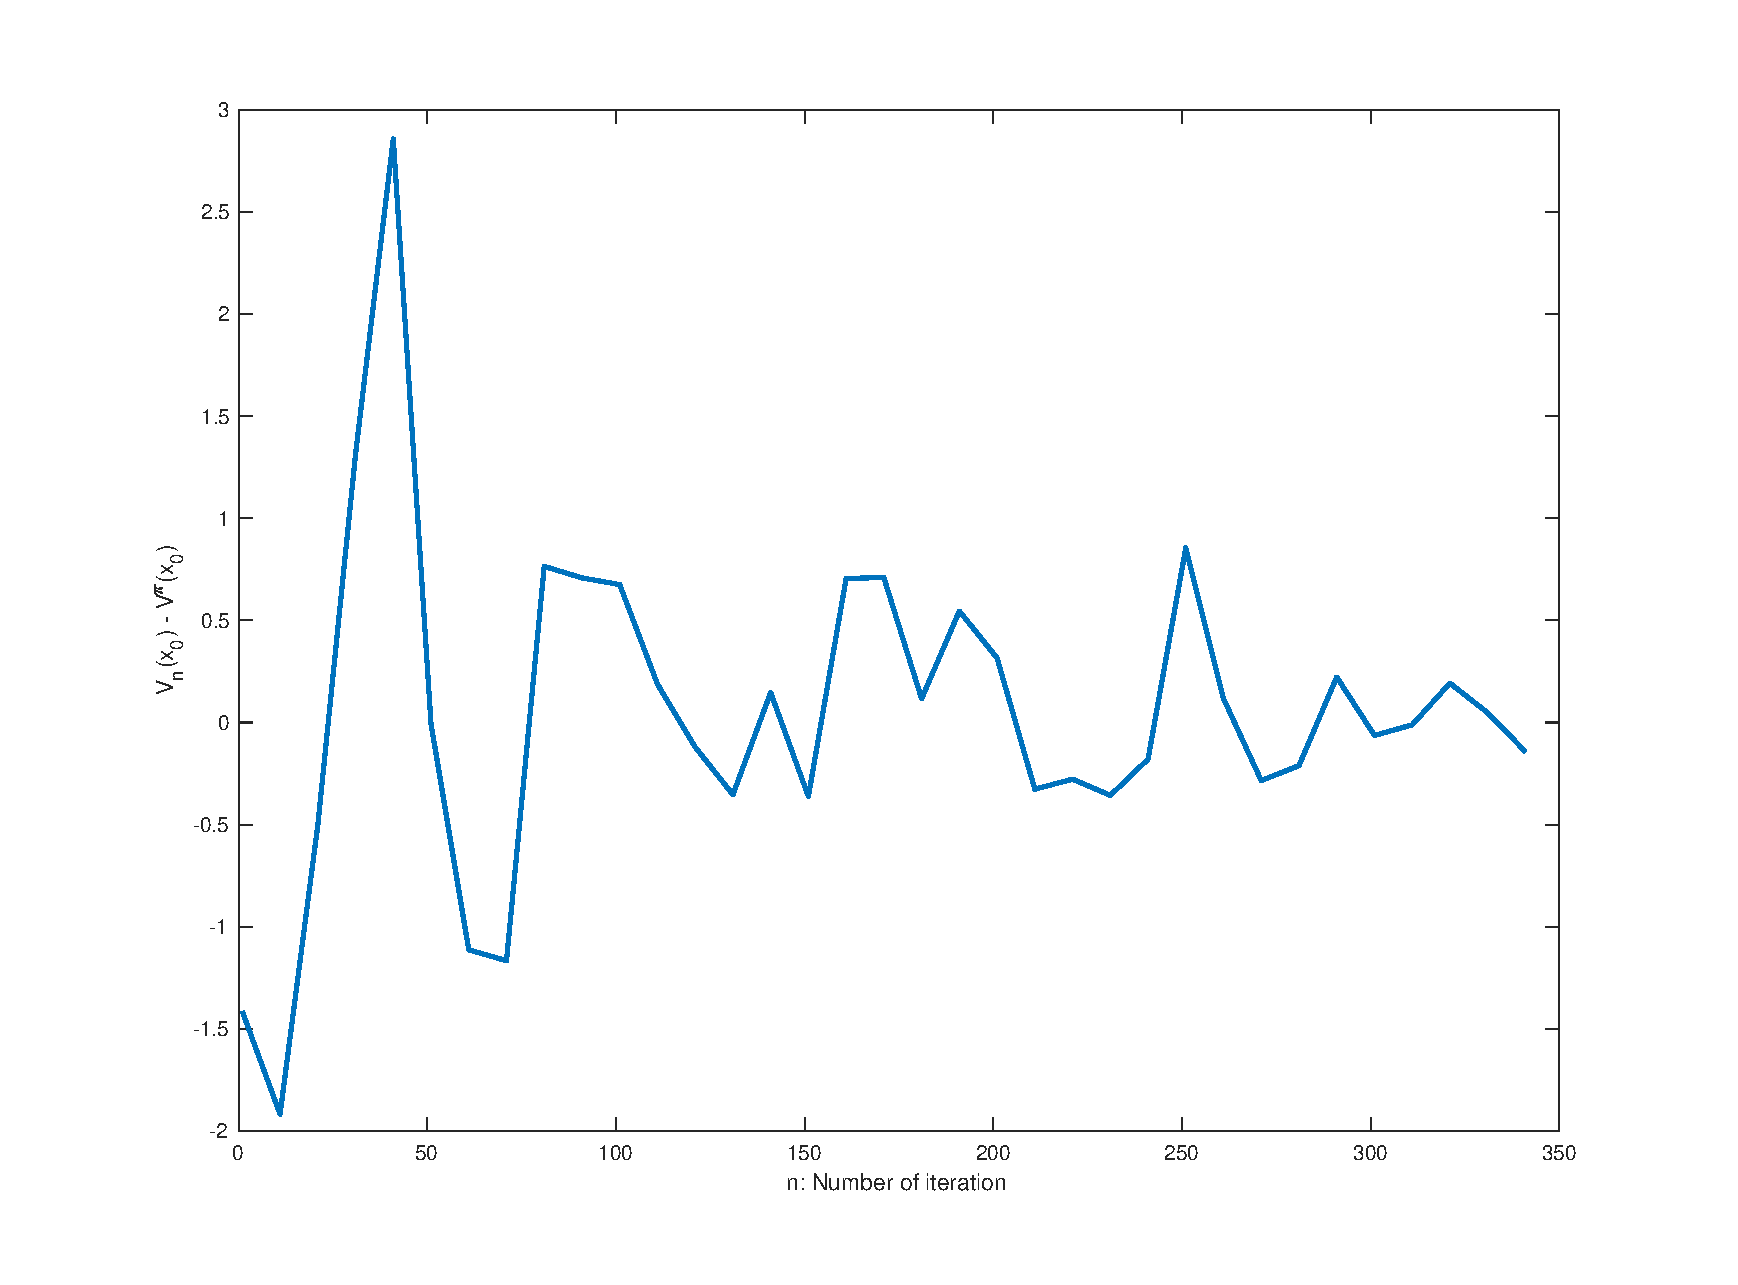
\includegraphics[width=13cm]{figures/Vn-Vpi.eps}
\caption{Plot of $V_{n}(x_{0}) - V^{\pi}(x_{0})$ with n increasing. We see that $V_{n}$ converge to $V^{\pi}$}    
\label{Vn-Vpi}
\end{figure}


\textbf{Q.3: Compute the optimal policy with the two dynamic programming method seen in class, Policy Iteration and Value Iteration.\\}

We implemented two functions: \verb|value_iteration.m| and \verb|policy_iteration|, that computer the optimal policy using those two methods. \\
Given the chosen parameters for the experiment (shown in Q1.) The Optimal policy is the following:

\begin{center}
	\begin{tabular}{ c | c | c  | c  | c  | c  | c  | c  | c  | c | c | c}
		 State & 1 & 2 & 3 & 4 & 5 & 6 & 7 & 8 & 9 & 10 & sick \\
		 \hline
		 Action & 1 & 1 & 1 & 1 & 1 & 1 &  2 & 2 & 2 & 2 & 1 \\
 	\end{tabular}
\end{center}

\textbf{Q.4: For both methods, plot $||V^{*} ? V_{k}||$ as a function of iteration k to compare the speed of convergence and discuss the relative merits of the two approaches.\\}

Figure \ref{vstar_vk} shows the convergence for the two methods in function of the number of iteration. We clearly see that Value Iteration take much more time to converge than the Policy Iteration. Actually Policy Iteration converge in a finite number of iteration (here 5), whereas Value Iteration seems to converge only asymptotically. However Policy Iteration is much more expensive as it needs an $eval\_policy$ step.\\

\begin{figure}[!h]
\centering
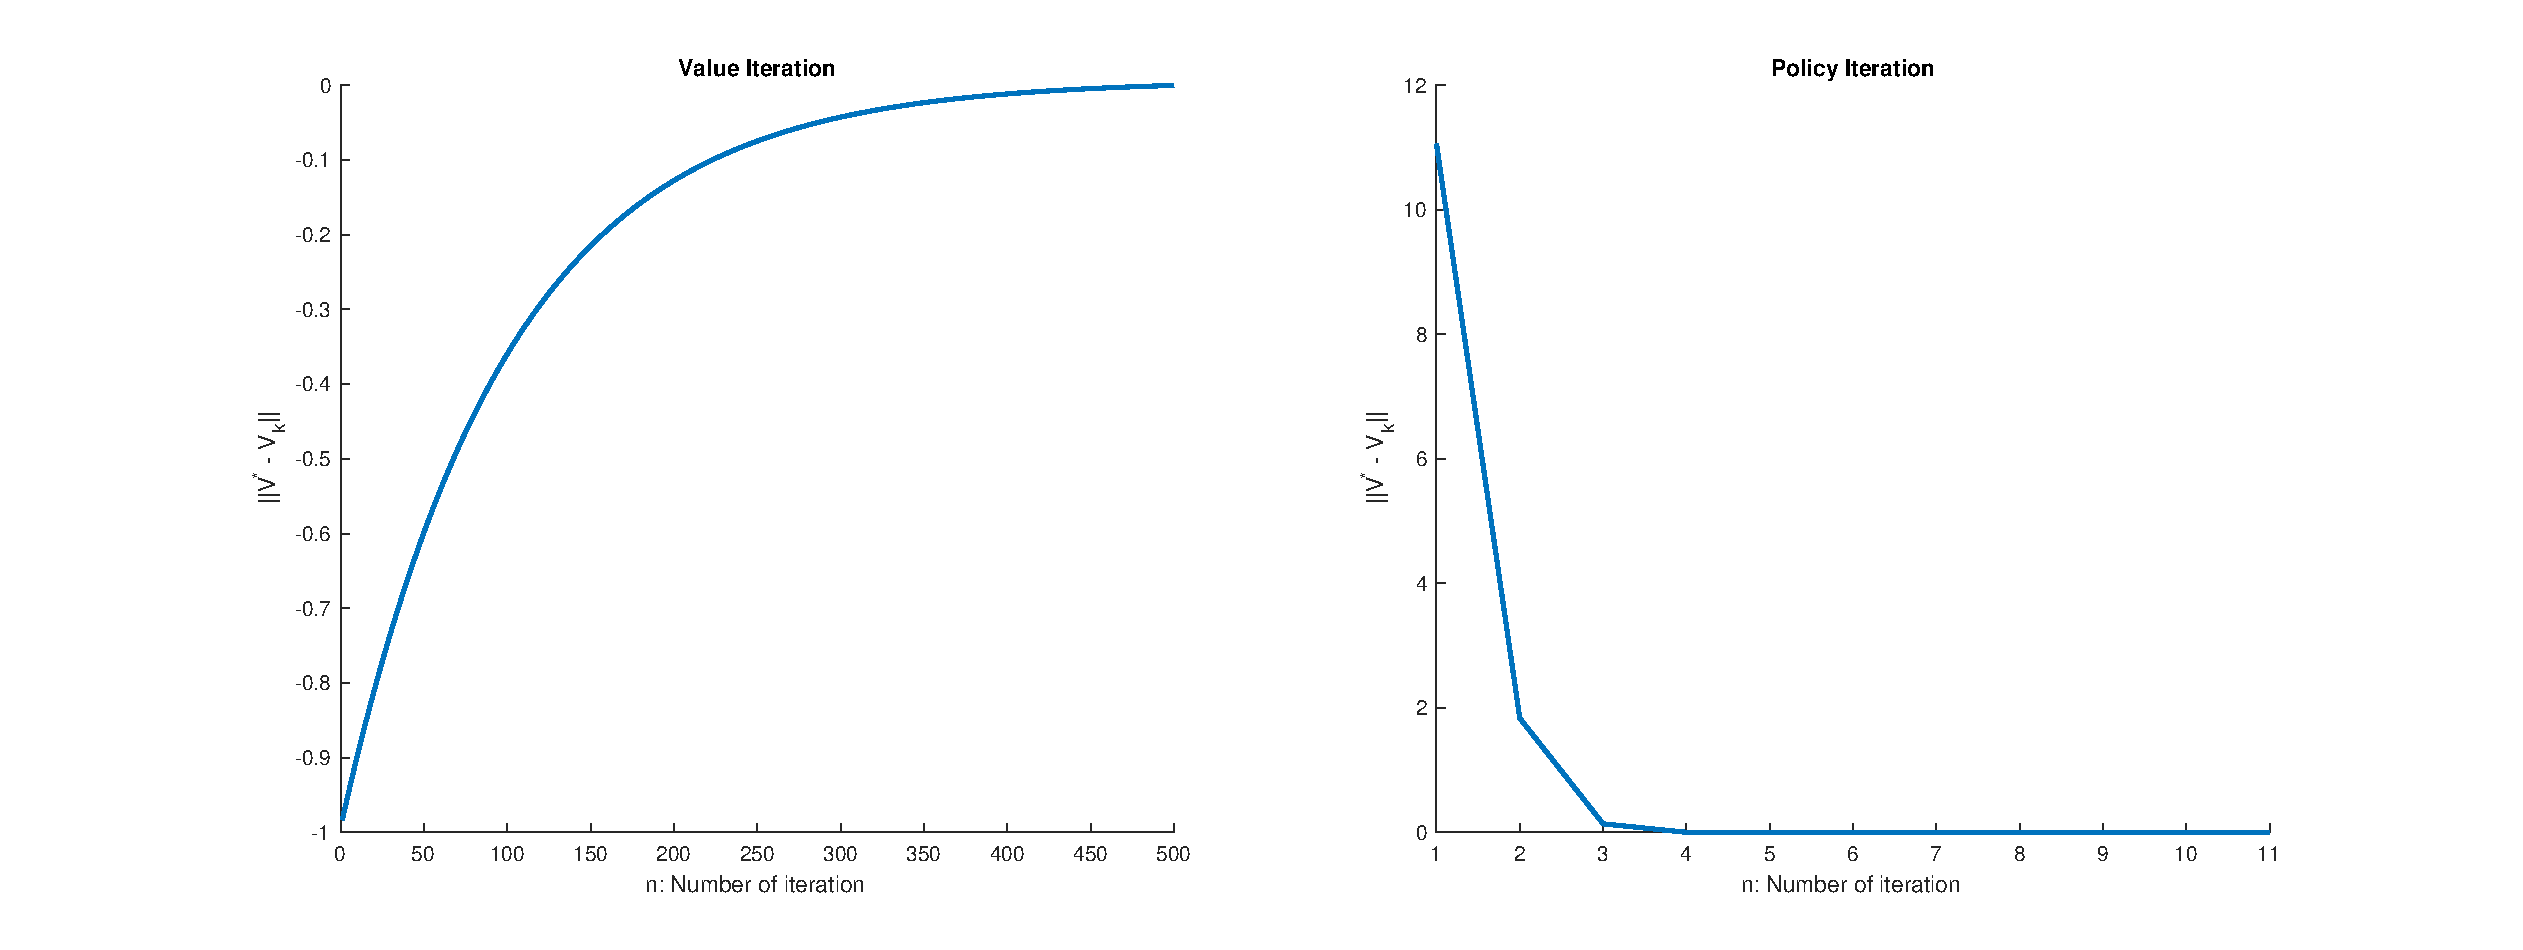
\includegraphics[width=16cm]{figures/vstar_vk.eps}
\caption{Plot of $||V^{*} - V_{k}||$ for increasing value of iteration $k$. Convergence for the Value Iteration method on the left, and Policy Iteration on the right.}    
\label{vstar_vk}
\end{figure}


\clearpage


%----------------------------------------------------------------------------------------
%	BIBLIOGRAPHY
%----------------------------------------------------------------------------------------

\bibliographystyle{apalike}

\bibliography{sample}

%----------------------------------------------------------------------------------------


\end{document}